\section{Preliminaries}

\subsection{Destributed SGD}
\begin{frame}
    \frametitle{Destributed SGD}
	\begin{figure}
		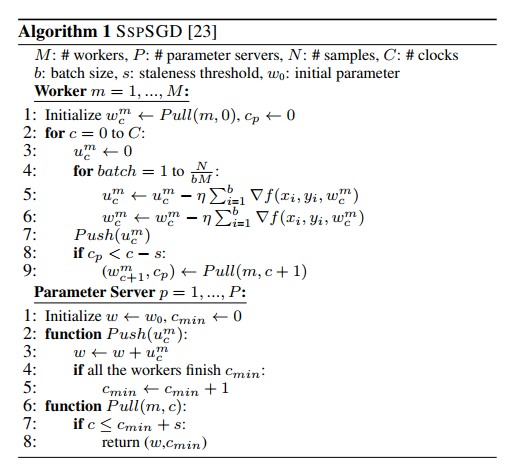
\includegraphics[scale=0.45]{figure/sgd.png}
	\end{figure}
\end{frame}

\subsection{Instroduction of existing systems}
\begin{frame}
    \frametitle{Instroduction of existing systems}
	\begin{itemize}
		\item BSP system: Bulk Synchronous Parallel. 
		\item ASP system: Asynchronous Parallel.
		\item SSP system: Stale Synchronous Parallel. 
	\end{itemize} 
\end{frame}
		
\subsection{Modeling Heterogeneous Clusters}
\begin{frame}
    \frametitle{HL}
	\begin{itemize}
		\item Decomposing the run time of worker into the computation time $t_{c}^{m}$, the transmission time $t_{t}^{m}$.
		\item The heterogeneous level of the cluster is measured by the speed gap between the fastest weorker and the slowest worker.
			\begin{itemize}
				\item $HL = \frac{t_{c}^{s}+t_{t}^{s}}{t_{c}^{f}+t_{t}^{f}}\qquad$
			\end{itemize}
	\end{itemize} 
\end{frame}

\subsection{Experiment on existing systems}
\begin{frame}
    \frametitle{Experiment}
	\begin{itemize}
		\item BSP:Spark, ASP:Petuum, SSP:Bosen. 
		\item They activate the sleep() function in 20\%workers to simulate the heterogeneous environment. 
	\end{itemize}
	\begin{figure}
		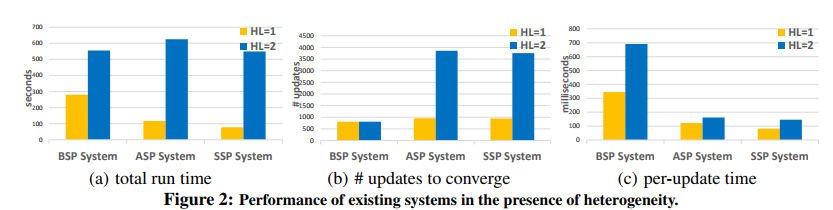
\includegraphics[scale=0.4]{figure/experiment_exist.png}
	\end{figure}
\end{frame}


